\section{Result}
\label{sec:analysis:result}



This sections presents the results of the estimates of the branching
fractions using the two methods presented earlier, and a test of lepton
universality based on the measured values of the leptonic branching
fractions.

\subsection{W branching fraction measurement}

The measurement of the branching fractions is carried out using both the
MLE and the semi-analytic method.  The specifics of both measurements
are described in Section~\ref{sec:method}.  The datasets used are common
to both categories, but the approach for how the branching fractions are
determined are substantially different.  One important distinction
between the two measurements is that the MLE method measures the
branching fraction simultaneously in all channels while the
semi-analytic approach measures the branching fractions separately in
different trigger and b-tag categories.  The resulting values for the
\PW branching fractions are shown in
Table~\ref{tab:results}.

\begin{table}[h]
    \centering
    \topcaption{Values of branching fractions determined in both
        analysis approaches and the PDG values.  Errors combine
        statisitcal and systematics uncertainties.
    \label{tab:results}}
    \begin{tabular}{l|c|c|c}
                   & semi-analytic          & MLE                   & PDG                  \\
    \hline                                                                 
    $\beta_{e}$    & $ (10.80 \pm 0.22) \%$ & $(10.8 \pm 0.11) \%$ & $(10.71 \pm 0.16)$ \% \\
    $\beta_{\mu}$  & $ (10.80 \pm 0.23) \%$ & $(10.8 \pm 0.08) \%$ & $(10.63 \pm 0.15)$ \% \\
    $\beta_{\tau}$ & $ (10.80 \pm 0.68) \%$ & $(10.8 \pm 0.19) \%$ & $(11.38 \pm 0.21)$ \% \\
    $\beta_{h}$    & $-- \pm --$            & $(67.4 \pm 0.26) \%$ & $(67.41 \pm 0.27)$ \% \\
    \end{tabular}
\end{table}


\subsection{Test of lepton universality (\textbf{WIP})}

Having established the method for estimating the branching fractions,
hypothesis tests can be carried out.  To do this, the profile likelihood
ratio is constructed assuming a null hypothesis of lepton universality
and two scenarios of unequal branching fractions for the alternative
hypothesis.  The two hypotheses that are tested are:


The test allows us to quantify p values that correspond to the values of
$q$ determined from fitting the data.  In order to do this, the pdf of
$q$ for both scenarios needs to be estimated.  Assuming regularity
conditions~\cite{Wilks}, the distributions will be $chi^{2}$ with one
d.o.f. for $q_{alt. 1}$ and two d.o.f. for $q_{alt. 2}$.  This has been
tested on 100 toy datasets and it is found that the distribution for
smaller excursions conform with Wilk's theorem (see
figure~\ref{fig:lu_test}.  Based on this, the distribution of the
likelihood ratio is well approximated by a $\chi^{2}_{k}$ distribution.

% \begin{figure}[h]
%     \begin{center}
%         \includegraphics[width=0.95\textwidth]{figures/lepton_universality_toys}
%         \caption{Distribution for the profile likelihood ratio for the two
%             hypothesis tests of interest based on toys data generated
%             from the Asimov dataset: \emph{left} the minimum NLL for
%             each evaluated toy dataset, and \emph{right} distribution for
%             $q_{alt. 1}$ and $q_{alt. 2}$.
%             \label{fig:lu_test}}
%     \end{center}
% \end{figure}



\subsection{Branching Ratio}

Test of lepton flavour universality (LFU) between electron and muons in 
weak section has been performed to unprecedented precision
in the past two decades. The tests have been carried out on both
colliders and fix target experiments. Their results are shown
in Table \ref{tbl:testlfuemu}. In general, the measurements
branching ratios between electron and muon agree very well with 
SM prediction.

% \input{section6/tables/emutest.tex}

In contract with agreement on LFU for $e$ and $\mu$ in weak section, LPU 
regarding $\tau$ versus $e$ and $\mu$, as is discussed in Chapter 1, 
is significantly challenged by 
measurements from ALEPH, DELPHI, OPAL and L3 with LEP e+e- collision, 
as well as Belle, Belle and LHCb with B meson decay.


Therefore, we are interesed in the ratio of $Br (W\to \tau \nu)$ with respect to electron
and muon channels,

\begin{equation}
    r = \frac{Br (W\to \tau \nu)}{Br (W\to l \nu)} , \text{ where } l=e,\mu
\end{equation}

based on the assumption that $Br (W\to \mu \nu) = Br( W\to e \nu )$, which
is well justified by the previous precision test of LFU between $e$ and $\mu$ in weak section.
This assumption is the same in Belle and BaBar measurements.

The key to the success of Belle and BaBar measurements is that $tau$ are reconstructed
by the same method as electron or muon, such that systematics regarding object
reconstruction and selection are cancelled.
Following this principle, we are measuring r in purely dilepton channels with muonic and electronic taus.
Comparing with hadronic taus, this avoids the systematic uncertainty related to hadronic tau efficiency
and misidentification.
By using leptonic taus, systematics regarding lepton reconstruction 
is canceled out to the first order, thus the precision of r is not limited systematically.

The evolved dilepton channels are $\mu\mu$, $ee$ and $e\mu$ with $n_j \geq 2$ and $n_b = 1,2$,
where $\mu\mu$, $ee$ also include $n_b = 0$ bin for Z background normalization purpose.
r is obtained by simultaneous fit to the pT spectrum of the trailing lepton in $\mu\mu$,
$ee$ and $e\mu$ channels. The methodology of this template fit is described in Section 5.3.
The result is in Eqn \ref{eqn:fitr}.

\begin{equation}
    \boxed{
    r = \frac{Br (W\to \tau \nu)}{Br (W\to l \nu)}
    = 1.000 \times \big[1 \pm 2.72\% \text{ (stat)} \pm 1.44\% \text{ (syst)} \big]
    }
    \label{eqn:fitr}
\end{equation}

The correlation matrix of the fit is shown in Fig \ref{fig:covr}.

The measurement of r using leptonic tau has small systematic uncertainty, thanks to the 
cancellation of reconstruction efficiency. The precision of r is statistically limited, 
which is expected to be improved when including 2017 data.


The improvement of r precision when including more channels is shown in
Fig \ref{fig:gain}. The gain of adding $e\mu$ and $\mu e$ channel is
significant, while adding $l \tau$ and $l4j$ channel is small.


\begin{figure}[p]
    \centering
    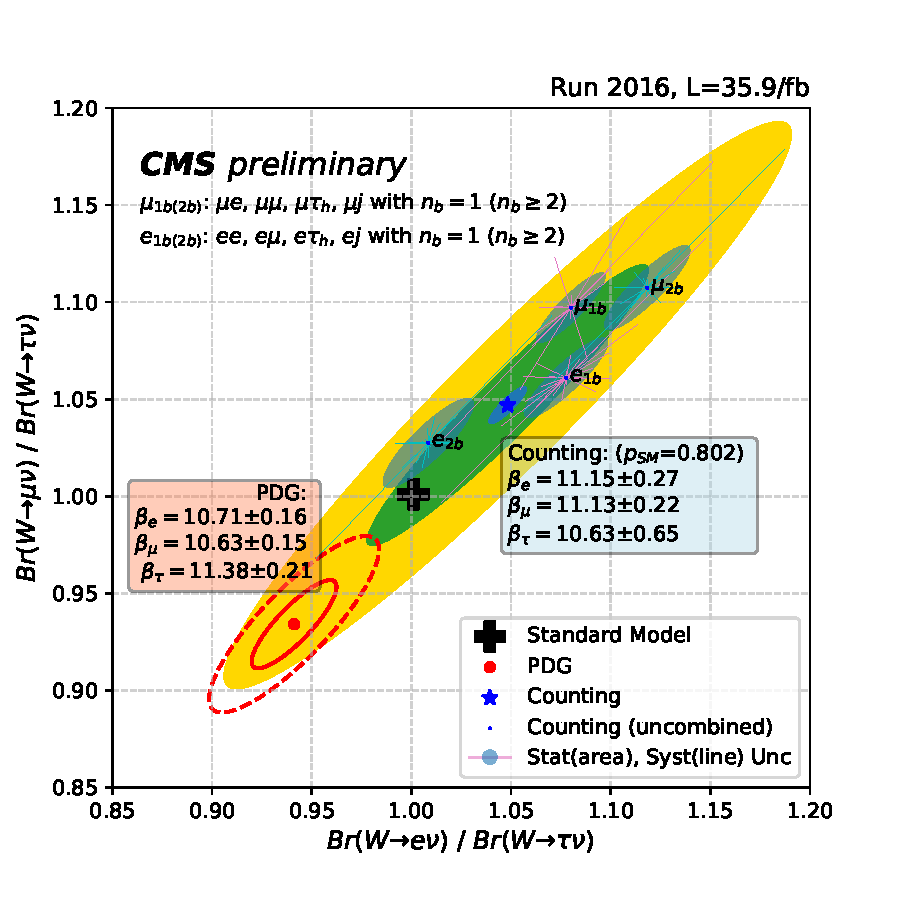
\includegraphics[width=14cm]{chapters/Analysis/sectionResult/figures/r2}
    \caption{Fitting the pT spectrum of trailing lepton in $ee$, $\mu\mu$ and $e\mu$ channel.
    The correlation matrix among r and systematic parameters.
    }
    \label{fig:covr}
\end{figure}